
\let\negmedspace\undefined
\let\negthickspace\undefined
\documentclass[journal]{IEEEtran}
\usepackage[a5paper, margin=10mm, onecolumn]{geometry}
%\usepackage{lmodern} % Ensure lmodern is loaded for pdflatex
\usepackage{tfrupee} % Include tfrupee package

\setlength{\headheight}{1cm} % Set the height of the header box
\setlength{\headsep}{0mm}     % Set the distance between the header box and the top of the text

\usepackage{gvv-book}
\usepackage{gvv}
\usepackage{cite}
\usepackage{amsmath,amssymb,amsfonts,amsthm}
\usepackage{algorithmic}
\usepackage{graphicx}
\usepackage{textcomp}
\usepackage{xcolor}
\usepackage{txfonts}
\usepackage{listings}
\usepackage{enumitem}
\usepackage{mathtools}
\usepackage{gensymb}
\usepackage{comment}
\usepackage[breaklinks=true]{hyperref}
\usepackage{tkz-euclide} 
\usepackage{listings}
% \usepackage{gvv}                                        
\def\inputGnumericTable{}                                 
\usepackage[latin1]{inputenc}                                
\usepackage{color}                                            
\usepackage{array}                                            
\usepackage{longtable}                                       
\usepackage{calc}                                             
\usepackage{multirow}                                         
\usepackage{hhline}                                           
\usepackage{ifthen}                                           
\usepackage{lscape}
\begin{document}

\bibliographystyle{IEEEtran}
\vspace{3cm}

\title{1.9.10}
\author{EE24BTECH11020 - Ellanti Rohith}
% \maketitle
% \newpage
% \bigskip
{\let\newpage\relax\maketitle}

\renewcommand{\thefigure}{\theenumi}
\renewcommand{\thetable}{\theenumi}
\setlength{\intextsep}{10pt} % Space between text and floats


\numberwithin{equation}{enumi}
\numberwithin{figure}{enumi}
\renewcommand{\thetable}{\theenumi}


\textbf{Question}:The distance between the points $\vec{A} \myvec{0\\6}$ and $\vec{B} \myvec{0\\-2}$ is \rule{1cm}{0.15mm} \vspace{.5em} \\  \\ \textbf{Solution:} We know that distance between two points $\vec{A}$ and $\vec{B}$ is $\sqrt{(\vec{A}-\vec{B})^\top (\vec{A}-\vec{B})}$ \\[1.5em]
	\begin{align}
\because
		\vec{A} - \vec{B} &= \myvec{0\\6} - \myvec{0\\-2} = \myvec{0\\8},		
\\[1.8em]
\sqrt{(\vec{A}-\vec{B})^\top (\vec{A}-\vec{B})} &= \sqrt{\myvec{0 & 8} \myvec{0\\8}} = \sqrt{0 + 64} = 8
	\end{align} 
	Thus, the desired distance is $\vec{A}$ and $\vec{B}$ is 8 units.
	\\\begin{figure}[h!]
   \centering 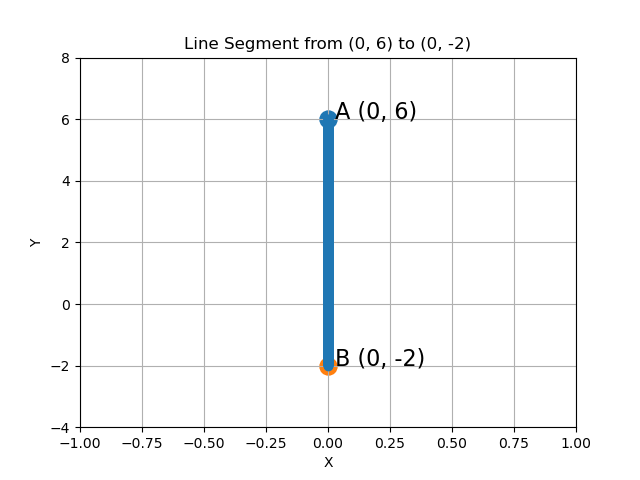
\includegraphics[width=0.7\linewidth]{figs/fig.png}
   \label{Plot of Vector AB}
   \end{figure}
	

\end{document}

